\chapter{Generating Test Cases}\label{ch:tests}

In this chapter, we show how to use occurrence graph grammars to generate test cases from (simply-typed) graph grammars that model systems. This approach can be used to generate tests for any graph grammar, in our examples however, we will use grammars that were built using the methodology presented in \cite{Junior2015} and \cite{BezerraWEIT2016}.

This methodology is a systematic, computer-aided way to extract graph grammars from use cases and other text-based requirement documents. Thus, by generating tests from these grammars, we are generating tests for the use cases where they came from.

Regarding the generation of test cases, we are interested in knowing whether each functionality is truly executable, i.e. whether all the rules that represent that functionality are applicable. If the functionality is not executable we want to know exactly what is the problem in te execution, if it is executable, we wnat to know:

\begin{enumerate}
\item the input data necessary for this functionality to execute, as well as the output data of a successful execution;

\item a characterization of the possible orderings in which all the rules can be applied to accomplish the functionality goals, together with some total orderings that respect this characterization and others that do not;

\item which are the valid (and invalid) intermediate states the system may assume.
\end{enumerate}

First, we present a brief overview of the methodology for extracting graph grammars from use cases, after what we present the process of generating the tests cases from the the grammars.

\section{Overview of the original methodology} \tinytodo{this entire subsection is a copy from the weit article, must be adapted to the needs of this work} A general format of a UC contains a set of sequential steps describing the successful interaction between the primary actor and the system towards the primary goal. A sequence of alternative steps are often included to represent exception flows. Pre- and post-conditions are also listed to indicate, respectively, conditions that must hold before and after the UC execution.

Figure~\ref{fig:tests:methodology} summarizes the methodology process, which is divided into four main phases:

\begin{figure}[!ht]
  \centering
  \fbox{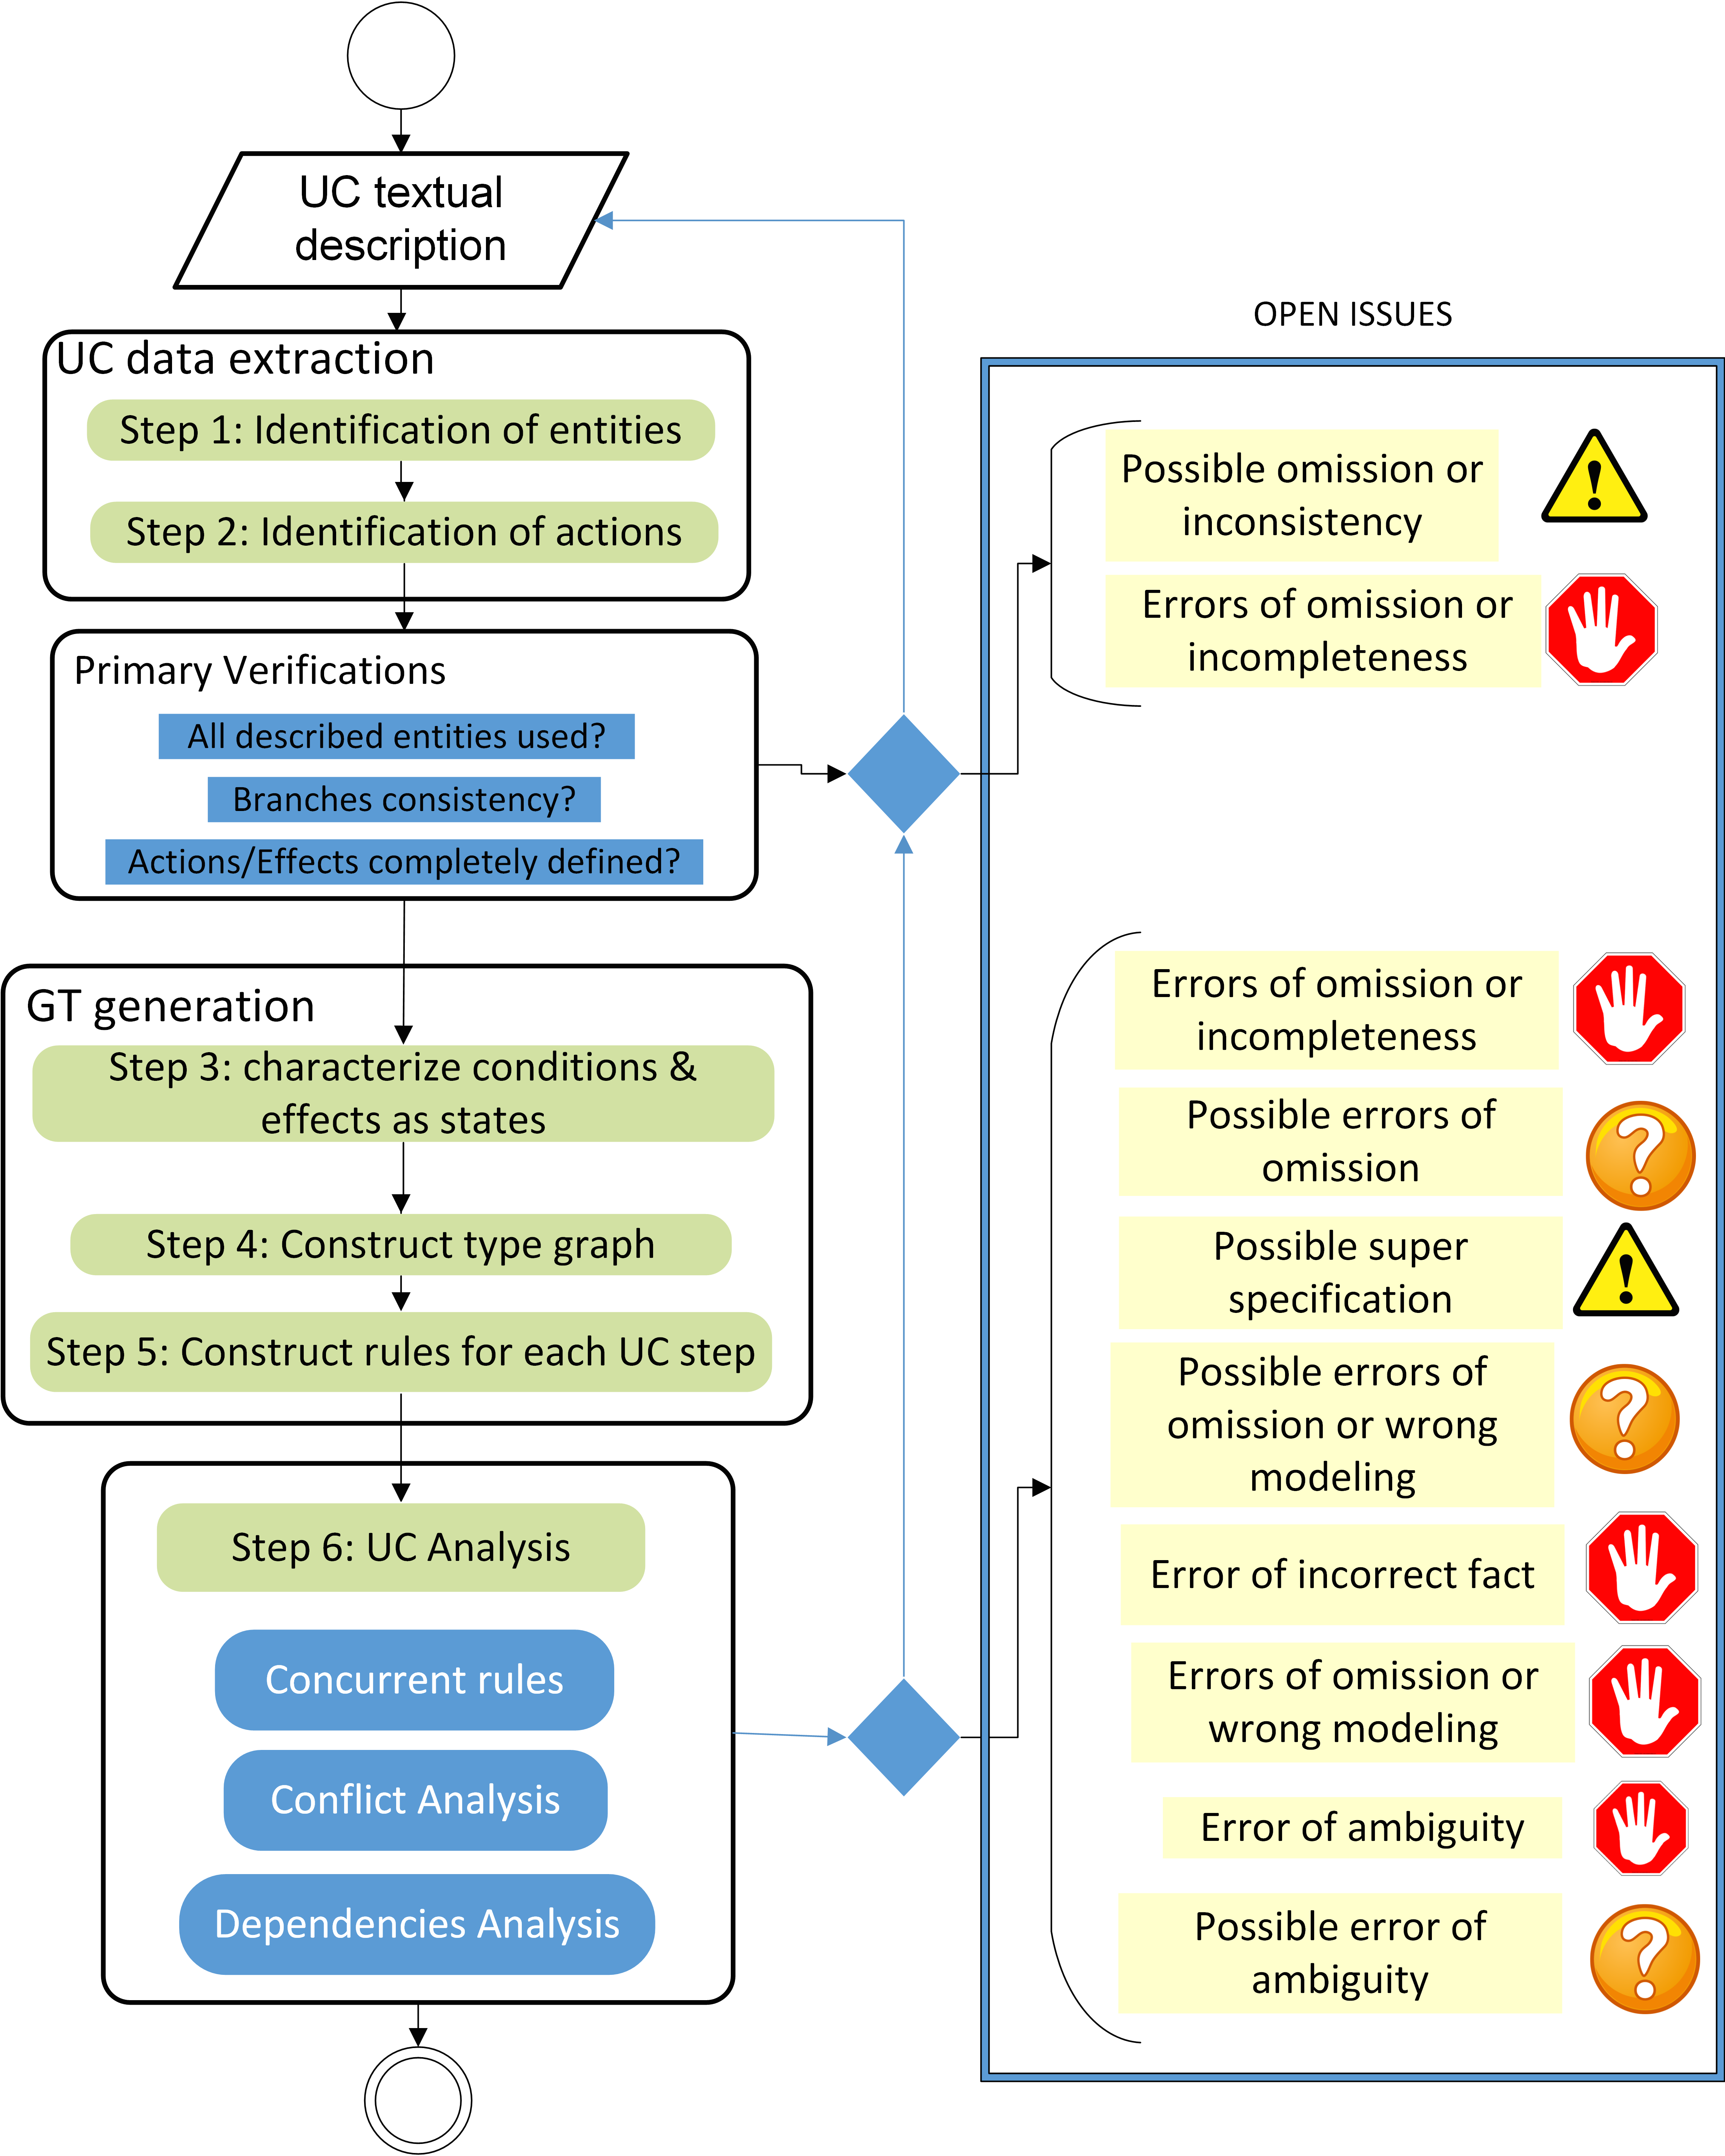
\includegraphics[scale=0.6]{images/generating-tests/methodology}}
  \caption{Overview of the methodology~\cite{Junior2015}.}\label{fig:tests:methodology}
\end{figure}

\begin{description}
  \item[Data Extraction:] where we identify entities and actions in the text of the UC that will be used to construct the model.
  \item[Primary Verifications:] where we look for problems such as entities or conditions that were found in the previous phase but are never used and also for actions and effects not clearly defined. As these problems might affect or even prevent the creation of the model, they have to be either solved by rewriting the UC or annotated as open issues to be resolved later on if they are not prohibitive to the model construction.
  \item[GT Generation:] where we construct the GT model by modelling conditions and effects as graphs, building a type graph and then modelling each step of the UC as transition rule from one state graph (the conditions) to other (the effect).
  \item[UC Analysis:] where we perform a series of automated verifications over the GT model to detect possible flaws in the UC. This is done by using the verigraph tool \tinytodo{generate DOI for the latest version of verigraph} and its concurrent rules, conflict and dependency analyses.
\end{description}

Figure~\ref{} shows a piece of the graph grammar extracted from the set of use cases presented in~\cite{Goins2007}. These use cases model an e-store, with basic functionalities such as \emph{browse catalogue, user registration, login, update user information, maintain shopping cart}, among others. The complete extracted grammar can be seen on appendix~\ref{app:marvel-grammar}.

\section{Generating Tests using Occurrence Graph Grammars}

Given a graph grammar \graphGrammar{} modelling a system $X$ with $n > 0$ functionalities, we want to generate a test case for each subset of rules $F_i \subseteq P$ $\forall i \in 1\ldots n$, where $F_i$ represents a complete functionality \tinytodo{feature} of the system $X$.

Together with the grammar $GG$ and its subsets of functionalities $F_i$, we will also need an \emph{input-output relation} $IO_i$ for each $F_i$, specifying the connections between the rules in $F_i$. This \emph{input-output relation} specifies which elements (nodes and edges) must be the same among the rules, as shown in example~\ref{ex:inout}.

\begin{example}[Input-Output Relations]\label{ex:inout}


\begin{figure}[!ht]
  \centering
  \fbox{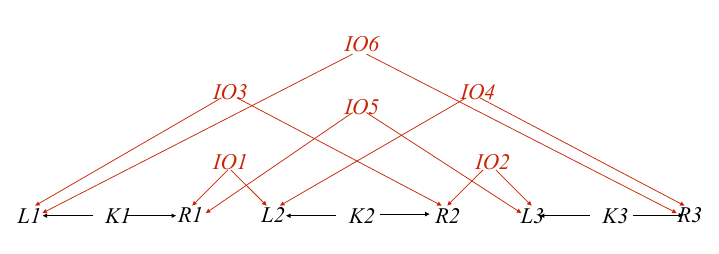
\includegraphics[scale=0.7]{images/generating-tests/inout}}
  \caption{Input-Output relation structure.}\label{fig:tests:inout}
\end{figure}

\end{example}

Given a grammar $GG$ modelling a system, its set of rules $P$, together with $F_i$ and $IO_i$, we generate as output:

\begin{enumerate}
\item an amalgamation (colimit) $OGG_i$ of rules for each $F_i$ with respect to $IO_i$
\item the initial and final graphs $I_i$ and $J_i$ of $OGG_i$, representing the input and output data of the functionality $F_i$
\item the conflict and dependency relations between rules \tinytodo{and the elements involved in the conflict / dependency}
\item restrictions over the ordering of elements existence and rules applicability
\item one or more total orderings that respect all relations and restrictions
\item one or more total orderings that do not respect the relations or restrictions
\end{enumerate}

First, the amalgamation of rules in $F_i$ w.r.t. $IO_i$ is responsible to ``glue'' the graphs of all rules in on single graph at the same that it identifies the items that come from different rules but are supposed to be the same element. 

If the result of this amalgamation is a \emph{core graph} according to definition~\ref{def:core-graph}, we can create a doubly-typed graph grammar $OGG_i$ that is also a strongly-safe grammar and therefore a candidate to be an occurrence graph grammar. Otherwise, there is more than one rule that deletes or creates
the same element, thus it is not possible to apply all rules of this functionality.

\diagram{
  & & & & IO_6\ar[dddrrrr]\ar[dddllll] & & & & &\\
  & IO_3\ar[ddl]\ar[ddrrrr] & & & & & & IO_4\ar[ddr]\ar[ddllll] & &\\
  & & IO_1\ar[d]\ar[dr] & & IO_5\ar[drr]\ar[dll] & & IO_2\ar[d]\ar[dl] & & & \\
  L_1\ar[dddrrrr] & K_1\ar[l]\ar[r] & R_1\ar[dddrr] & L_2\ar[dddr] & K_2\ar[l]\ar[r] & R_2\ar[dddl] & L_3\ar[dddll] & K_3\ar[l]\ar[r] & R_3\ar[dddllll] & \ldots\ar[dddlllll]\\
  & & & & & & & & & \\
  & & & & & & & & & \\
  In\ar[rrrr] & & & & Occ & & & & Out\ar[llll] &
}

\begin{figure}[!ht]
  \centering
  \fbox{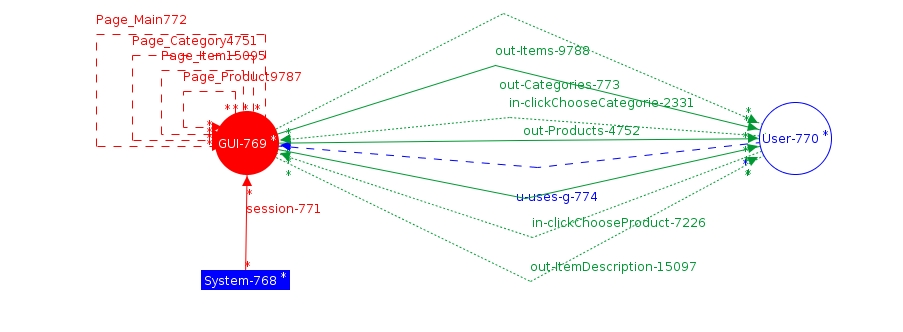
\includegraphics[scale=0.7]{images/generating-tests/colimit}}
  \caption{Amalgamation (colimit) of rules according to the IO relation.}\label{fig:tests:colimit}
\end{figure}

\begin{example}[Amalgamation example]\label{ex:amalgamation}
\end{example}

After identifying that $OGG_i$ is in fact a strongly-safe graph grammar, we can extract the initial and final graphs of $OGG_i$ by removing from the core graph the created and deleted elements, respectively. If they are valid graphs, we have the input and output data for the test case. Otherwise, if they have dangling edges, it is not possible to apply all rules of the functionality, since it would begin in or lead to an inconsistent state.

\begin{example}[Initial and Final Graphs Example]
\end{example}

Once the previous verifications were successful, we can build the occurrence relation (and any other relation discussed on chapter~\ref{ch:process}) to verify if $OGG_i$ can really be an occurrence graph grammar. If no abstract dependencies or conflicts are found, then the concrete relations are sufficient to do this verification, thus we simply need to check if there is a total ordering compatible with the relations.

\begin{example}[Occurence Relation]
\end{example}

If the set $R$ of \emph{occurrence relation restrictions} is not empty, we also need to check if there is a total ordering of the occurrence relation that respects these restrictions.

As this seems to be a hard problem, in the complexity sense, we left this last implementation as a future work. However, we still use the restrictions to generate a set of tests regarding the consistency of the system states.

In our case estudies, no such situation was found. We believe that it happens because we used grammars extracted from real use cases, where usually there are (possibly many) sequential connections between the actions, which forces the rules to be connected via the \emph{occurence relation} and avoids abstract restrictions.

\section{Building test cases with Verigraph}

More specific usability details can be found on the Verigraph tutorial, whose current version is presented on appendix~\ref{app:tutorial}.
